\chapter{Dérivation}

\section{Nombre dérivé}

\subsection{Taux de variation et nombre dérivé}

\begin{definition}[Taux de variation]
	Soit $f$ une fonction définie sur un intervalle $I$

	Soient $x_A$ et $h$ deux réels tels que $h\neq 0$, $x_A \in I$ et $\pa{x_A+h} \in I$.

	Le \textbf{taux de variation} de $f$ entre $x_A$ et $\pa{x_A+h}$ est le nombre :
	\[
		\dfrac{f(x_A+h)-f(x_A)}{h}
	\]

	\begin{center}
		\begin{tikzpicture}[>=Stealth,scale=0.9]
			\clip (-1.8,-1.5) rectangle (7.8,6);
			\draw[->, thick] (-1,0) -- (7,0) node[below left] {$x$};
			\draw[->, thick] (0,-1) -- (0,5.5) node[below left] {$y$};
			\node[below left] at (0,0) {$0$};
			\draw[domain=0.5:6.5, smooth, variable=\x, line width=1.5pt, blue] plot ({\x}, {0.15*(\x)^2 + 0.5});
			\node[blue, above right] at (4.8, 5.0) {$\mathcal{C}_f$};
			\def\a{2}\def\h{3}
			\pgfmathsetmacro{\aplusin}{\a+\h}
			\pgfmathsetmacro{\fa}{0.15*(\a)^2 + 0.5}
			\pgfmathsetmacro{\faplus}{0.15*(\aplusin)^2 + 0.5}
			\coordinate (A) at (\a, \fa);
			\coordinate (M) at (\aplusin, \faplus);
			\draw[dashed, gray, thick] (A) -- (\a, 0) node[below, black] {$a$};
			\draw[dashed, gray, thick] (M) -- (\aplusin, 0) node[below, black] {$a+h$};
			\draw[dashed, gray, thick] (A) -- (0, \fa) node[left, black] {$f(a)$};
			\draw[dashed, gray, thick] (M) -- (0, \faplus) node[left, black] {$f(a+h)$};
			\draw[domain=0.5:6.5, smooth, variable=\x, line width=1.2pt, red!80!black] plot ({\x}, {(\faplus-\fa)/\h * (\x - \a) + \fa}) node[right] {$(AM)$};
			\draw[->, thick, green!50!black] (A) -- (\aplusin, \fa) node[midway, below] {$h$};
			\draw[->, thick, green!50!black] (\aplusin, \fa) -- (M) node[midway, right] {$f(a+h)-f(a)$};
			\fill[black] (A) circle (2pt) node[above left] {$A$};
			\fill[black] (M) circle (2pt) node[above left] {$M$};
		\end{tikzpicture}
	\end{center}
\end{definition}

\begin{definition}[Nombre dérivé]
	Lorsque le taux de variation tend vers un réel quand $h$ tend vers $0$, on dit que $f$ admet un \textbf{nombre dérivé} en $x_A$. Ce nombre dérivé est noté $f^\prime(x_A)$.

	On dit aussi que $f$ est \textbf{dérivable} en $x_A$, et on a :
	\[
		f^\prime(x_A) = \lim_{h \to 0} \dfrac{f(x_A+h)-f(x_A)}{h}
	\]

	\begin{center}
		\begin{tikzpicture}[>=Stealth,scale=0.9]
			\clip (-1.6,-1.5) rectangle (7.6,6);
			\draw[->, thick] (-1,0) -- (7,0) node[below left] {$x$};
			\draw[->, thick] (0,-1) -- (0,5.5) node[below left] {$y$};
			\node[below left] at (0,0) {$0$};
			\draw[domain=0.3:5.5, smooth, variable=\x, line width=1.5pt, blue] plot ({\x}, {0.15*(\x)^2 + 0.5});
			\node[blue, above right] at (4.8, 5.0) {$\mathcal{C}_f$};
			\def\a{2}
			\pgfmathsetmacro{\fa}{0.15*(\a)^2 + 0.5}
			\foreach \b in {2.8,3.6,4.4,5.2}{
					\pgfmathsetmacro{\fb}{0.15*(\b)^2 + 0.5}
					\pgfmathsetmacro{\cb}{(\fb-\fa)/(\b-\a)}
					\pgfmathsetmacro{\pb}{\fb - \cb*\b}
					\draw[domain=0.3:5.5, smooth, variable=\x, line width=1pt, red!80!black, opacity=0.3] plot ({\x}, {\cb * \x + \pb) });
					\draw[dashed, red, thick,opacity=0.6] (\b , \fb) -- (\b, 0);
					\fill[black,opacity=0.6] (\b, \fb) circle (2pt);
				}
			\node[font=\footnotesize, opacity=0.6, below] at (5.2 , 0) {$x_A+h$};
			\pgfmathsetmacro{\fprime}{0.3*\a}
			\coordinate (A) at (\a, \fa);
			\draw[dashed, gray, thick] (A) -- (\a, 0) node[below, black] {$x_A$};
			\draw[dashed, gray, thick] (A) -- (0, \fa) node[left, black] {$f(x_A)$};
			\draw[domain=0.3:5.5, smooth, variable=\x, line width=1.2pt, red!80!black] plot ({\x}, {\fprime * (\x - \a) + \fa});
			\draw[->, thick, green!50!black] (\a, \fa) -- (\a+2, \fa) node[midway, below,fill=white] {$1$};
			\draw[->, thick, green!50!black] (\a+2, \fa) -- (\a+2, {\fa + \fprime*2}) node[midway, right,fill=white] {$f^\prime(x_A)$};
			\fill[black] (A) circle (2pt) node[above left] {$A$};
		\end{tikzpicture}
	\end{center}
\end{definition}

\begin{ex}[Calculer un nombre dérivé à l'aide du taux de variation]
	Soit $f$ la fonction définie sur $\R$ par $f(x) = x^2$.

	On cherche à calculer le nombre dérivé de $f$ en $3$.

	\begin{itemize}
		\item On calcule le taux de variation pour $x_A=3$ en fonction de $h$ :
		      \[
			      \def\arraystretch{2}
			      \begin{array}{rcl}
				      \dfrac{f(3+h)-f(3)}{h} & = & \dfrac{(3+h)^2 - 3^2}{h}        \\
				                             & = & \dfrac{9 + 6h + h^2 - 9}{h}     \\
				                             & = & \dfrac{6h + h^2}{h} \qquad= 6+h
			      \end{array}
		      \]
		\item On fait tendre $h$ vers $0$ : le taux tend vers $6$ quand $h$ tend vers $0$.
	\end{itemize}

	Donc $6$ est le nombre dérivé de $f(x)=x^2$ en $3$, et on note $f^\prime(3) = 6$.
\end{ex}

\section{Tangente à une courbe}

\subsection{Définition et coefficient directeur}

\begin{definition}[Tangente à une courbe]
	Si $f$ est dérivable en $x_A$, la \textbf{tangente} en $A$ à la courbe représentative de $f$ au point d'abscisse $x_A$ est la droite obtenue comme position limite des droites sécantes à la courbe passant par le point d'abscisse $x_A$ et le point d'abscisse $x_A+h$.

	\begin{center}
		\begin{tikzpicture}[>=Stealth,scale=0.9]
			\clip (-1.2,-1) rectangle (6,5);
			\draw[->, thick] (-1,0) -- (6,0) node[below left] {$x$};
			\draw[->, thick] (0,-1) -- (0,5) node[below left] {$y$};
			\node[below left] at (0,0) {$0$};
			\draw[domain=-0.5:5.3, smooth, variable=\x, line width=1.5pt, blue] plot ({\x}, {0.15*(\x)^3 - 0.9*(\x)^2 + 1.2*\x + 1});
			\node[blue, above right] at (4.5, 4.2) {$\mathcal{C}_f$};
			\draw[domain=-0.5:3, smooth, variable=\x, line width=1pt, red!80!black] plot ({\x}, {-0.15*(\x - 1) + 1.45});
			\draw[dashed, domain=-4:8, smooth, variable=\x, red!80!black] plot ({\x}, {-0.15*(\x - 1) + 1.45});
			\fill[black] (1, 1.45) circle (2pt) node[above] {$B$};
			\draw[domain=1:5, smooth, variable=\x, line width=1pt, violet!80!black] plot ({\x}, {-0.15*(\x - 3) + 0.55});
			\draw[dashed, domain=-4:8, smooth, variable=\x, violet!80!black] plot ({\x}, {-0.15*(\x - 3) + 0.55});
			\fill[black] (3, 0.55) circle (2pt) node[below] {$C$};
			\draw[domain=3.7:5.3, smooth, variable=\x, line width=1pt, green!50!black] plot ({\x}, {2.2125*(\x - 4.5) + 1.84375});
			\draw[dashed, domain=2.5:6.2, smooth, variable=\x, green!50!black] plot ({\x}, {2.2125*(\x - 4.5) + 1.84375});
			\fill[black] (4.5, 1.84375) circle (2pt) node[left] {$D$};
			\draw[domain=-1:1, smooth, variable=\x, line width=1pt, orange!80!black] plot ({\x}, {1.2*\x + 1});
			\draw[dashed, domain=-4:8, smooth, variable=\x, orange!80!black] plot ({\x}, {1.2*\x + 1});
			\fill[black] (0, 1) circle (2pt) node[above left] {$A$};
		\end{tikzpicture}
	\end{center}
\end{definition}

\begin{prop}[Coefficient directeur de la tangente]
	Soit $f$ une fonction dérivable en $x_A$.

	La tangente $T$ à la courbe $\Cf$ au point $A$ d'abscisse $x_A$ :
	\begin{itemize}
		\item \ldots passe par le point $A\coordl{x_A}{f(x_A)}$ ;
		\item \ldots a pour coefficient directeur le nombre dérivé $f^\prime(x_A)$.
	\end{itemize}

	On retient ainsi que :
	\[
		f^\prime(x_A) = \text{coef. dir. de la tangente en } A
	\]

	\begin{center}
		\begin{tikzpicture}[>=Stealth]
			\def\xa{2.9}
			\pgfmathdeclarefunction{f}{1}{\pgfmathparse{0.15*(#1+1)^3 - 0.9*(#1+1)^2 + 1.2*(#1+1)+0.7} }
			\pgfmathdeclarefunction{fprime}{1}{ \pgfmathparse{0.45*(#1+1)^2 - 1.8*(#1+1) + 1.2} }
			\pgfmathsetmacro{\fa}{f(\xa)}
			\pgfmathsetmacro{\fprime}{fprime(\xa)}
			\coordinate (A) at (\xa, \fa);
			\clip (-1.5,-1) rectangle (6,3);
			\draw[->, thick] (-1,0) -- (6,0) node[below left] {$x$};
			\draw[->, thick] (0,-1) -- (0,3) node[below left] {$y$};
			\node[below left] at (0,0) {$0$};
			\node[blue, above left] at ( {\xa + 0.8}, {f(\xa + 0.8)}) {$\mathcal{C}_f$};
			\draw[domain=-1.2:5.2, smooth, variable=\x, line width=1.5pt, blue] plot ({\x}, {f(\x)});
			\draw[domain=1.2:4.8, smooth, variable=\x, line width=1.2pt, red!80!black] plot ({\x}, {\fprime * (\x - \xa) + \fa}) node[above right] {$T$};
			\draw[dashed, gray, thick] (A) -- (\xa, 0) node[below, black] {$x_A$};
			\draw[dashed, gray, thick] (A) -- (0, \fa) node[left, black, fill=white] {$f(x_A)$};
			\draw[->, thick, green!50!black] (\xa, \fa) -- (\xa+1.5, \fa) node[midway, below] {$1$};
			\draw[->, thick, green!50!black] (\xa+1.5, \fa) -- (\xa+1.5, {\fa + \fprime*1.5}) node[midway, right] {$f'(x_A)$};
			\fill[black] (A) circle (2.5pt) node[above left] {$A$};
		\end{tikzpicture}
	\end{center}
\end{prop}

\subsection{Équation de la tangente}

\begin{prop}[Équation réduite de la tangente]
	Soit $f$ une fonction définie et dérivable sur $I$.

	La tangente à la courbe représentative de $f$ au point d'abscisse $x_A$ a pour équation :
	\[
		y = f^\prime(x_A)(x-x_A) + f(x_A)
	\]
\end{prop}

\begin{ex}[Calculer l'équation réduite de la tangente en un point]
	On considère la fonction $f$ définie sur $\R$ par $f(x) = x^2+2$.

	Déterminons l'équation réduite de la tangente à sa courbe représentative au point d'abscisse $x_A = 1$.

	\begin{enumerate}
		\item \textbf{Calcul de l'ordonnée du point de contact $f(x_A)$ :}
		      \[
			      f(1) = 1^2 + 2 = 1 + 2 = 3
		      \]

		      Le point de contact a pour coordonnées $A\coordl{1}{3}$.

		\item \textbf{Calcul du nombre dérivé $f^\prime(1)$ à l'aide du taux de variation :}

		      On calcule le taux de variation de $f$ entre $1$ et $1+h$ (avec $h \neq 0$) :
		      \[
			      \def\arraystretch{2}
			      \begin{array}{rcl}
				      \dfrac{f(1+h)-f(1)}{h} & = & \dfrac{\left((1+h)^2 + 2\right) - (1^2 + 2)}{h}             \\
				                             & = & \dfrac{1 + 2h + h^2 + 2 - 3}{h}                             \\
				                             & = & \dfrac{2h + h^2}{h} \qquad = \dfrac{h(2+h)}{h} \qquad = 2+h
			      \end{array}
		      \]

		      Lorsque $h$ tend vers $0$, le taux de variation tend vers $2$.

		      On en déduit que $f^\prime(1) = 2$. Le coefficient directeur de la tangente est donc égal à $2$.

		\item \textbf{Détermination de l'équation de la tangente :}

		      L'équation réduite de la tangente en $x_A = 1$ est donnée par la formule :
		      \[
			      y = f^\prime(1)(x - 1) + f(1)
		      \]

		      En injectant nos valeurs ($x_A = 1$, $f(1) = 3$ et $f^\prime(1) = 2$) :
		      \[
			      \begin{array}{lcl}
				      y & = & 2 \times (x - 1) + 3 \\
				        & = & 2x - 2 + 3           \\
				        & = & 2x + 1
			      \end{array}
		      \]
	\end{enumerate}

	L'équation réduite de la tangente à la courbe de $f$ au point d'abscisse $1$ est donc $y = 2x + 1$.

	\begin{center}
		\begin{tikzpicture}[>=Stealth, y=5mm, scale=1.3]
			\def\xmin{-1.7}\def\xmax{3}
			\def\ymin{-1.5}\def\ymax{7.5}\def\xa{1}
			\pgfmathdeclarefunction{f}{1}{\pgfmathparse{(#1)^2 + 2}}
			\pgfmathdeclarefunction{fprime}{1}{\pgfmathparse{2*(#1)}}
			\pgfmathsetmacro{\fa}{f(\xa)}
			\pgfmathsetmacro{\fp}{fprime(\xa)}
			\clip (\xmin,\ymin) rectangle (\xmax,\ymax);
			\draw[->, thick] (\xmin,0) -- (\xmax,0) node[below left] {$x$};
			\draw[->, thick] (0,\ymin) -- (0,\ymax) node[below left] {$y$};
			\node[below left] at (0,0) {$0$};
			\coordinate (A) at (\xa, \fa);
			\draw[domain=-1.5:2.2, smooth, variable=\x, line width=1.5pt, blue] plot ({\x}, {f(\x)});
			\node[blue, left] at ({-1}, {f(-1)}) {$\mathcal{C}_f$};
			\draw[domain=-0.8:2.2, smooth, variable=\x, line width=1.2pt, red!80!black] plot ({\x}, {\fp * (\x - \xa) + \fa}) node[right] {$T$};
			\draw[dashed, gray, thick] (A) -- (\xa, 0) node[below, black] {$1$};
			\draw[dashed, gray, thick] (A) -- (0, \fa) node[left, black] {$4$};
			\draw[->, thick, green!50!black] (\xa, \fa) -- (\xa+1, \fa) node[midway, below] {$1$};
			\draw[->, thick, green!50!black] (\xa+1, \fa) -- (\xa+1, {\fa + \fp*1}) node[midway, right] {$2$};
			\fill[black] (A) circle (2pt) node[above left] {$A$};
			\fill[black] (0,{\fa-\fp*\xa}) circle (2pt) node[left] {$1$};
		\end{tikzpicture}
	\end{center}
\end{ex}

\section{Fonction dérivée et dérivées de fonctions usuelles}

\subsection{Fonction dérivée}

\begin{definition}[Fonction dérivée]
	Soit $f$ une fonction définie sur un intervalle $I$.

	La fonction $f$ est dite dérivable sur $I$ si elle est dérivable en tout réel $x$ de $I$.

	La fonction qui, à tout $x\in I$, associe le nombre dérivé $f^\prime(x)$, est appelée \textbf{fonction dérivée} de $f$.

	Cette fonction est notée $f^\prime$.
\end{definition}

\subsection{Dérivées des fonctions usuelles}

\begin{prop}[Dérivées de fonctions usuelles]
	Ce tableau indique les fonctions dérivées des fonctions les plus souvent rencontrées :
	\[
		\def\arraystretch{1.7}
		\begin{array}{|l|c|c|c|c|} \hline
			\ccg f(x)  & k~(k\in\R) & x & x^2 & x^3  \\ \hline
			\ccg f'(x) & 0          & 1 & 2x  & 3x^2 \\ \hline
		\end{array}
	\]
\end{prop}

\subsection{Opérations sur les fonctions dérivables}

\begin{prop}[Somme de fonctions]
	Soient $u$ et $v$ deux fonctions définies et dérivables sur un intervalle $I$.

	Alors $u+v$ est définie et dérivable sur $I$ et :
	\[
		(u+v)' = u' + v'
	\]

	La dérivée d'une somme est la somme des dérivées.
\end{prop}

\begin{prop}[Multiplication par un nombre réel]
	Soit $u$ une fonction définie et dérivable sur un intervalle $I$ et $k$ un nombre réel.

	Alors $ku$ est définie et dérivable sur $I$ et :
	\[
		(ku)' = k u'
	\]

	Si une fonction est multipliée par une constante, celle-ci est conservée lors de la dérivation.
\end{prop}
\begin{ex}
	Soit $f$ la fonction définie sur $\R$ par :
	\[
		f(x) = 6x^2 + 1
	\]

	En appliquant les formules de dérivation et les opérations sur les fonctions :
	\[
		\def\arraystretch{1.5}
		\begin{array}{rccccl}
			f(x)       & = & 6 \times & x^2 & + & 1                              \\
			\iff f'(x) & = & 6 \times & 2x  & + & 0 \qquad\iff f^\prime(x) = 12x
		\end{array}
	\]
\end{ex}

\begin{ex}
	Soit $f$ la fonction définie sur $\R$ par :
	\[
		f(x) = 3x^3 - 5x^2 + 2x - 7
	\]

	En appliquant les formules de dérivation et les opérations sur les fonctions :
	\[
		\def\arraystrech{1.5}
		\begin{array}{rccccccccccl}
			f(x)       & = & 3 \times & x^3  & - & 5 \times & x^2 & + & 2 \times & x & - & 7                                        \\
			\iff f'(x) & = & 3 \times & 3x^2 & - & 5 \times & 2x  & + & 2 \times & 1 & - & 0 \qquad\iff f^\prime(x)= 9x^2 - 10x + 2
		\end{array}
	\]
\end{ex}

\section{Étude des variations d'une fonction}

\begin{prop}[Lien entre dérivée et variations]
	Soit $f$ une fonction définie et dérivable sur un intervalle $I$.
	\begin{itemize}
		\item Si $f^\prime(x) \geq 0$ pour tout $x \in I$, alors $f$ est \textbf{croissante} sur $I$.
		\item Si $f^\prime(x) \leq 0$ pour tout $x \in I$, alors $f$ est \textbf{décroissante} sur $I$.
	\end{itemize}
\end{prop}

\begin{methode}[Étudier les variations d'une fonction]
	Pour étudier le sens de variation d'une fonction $f$ dérivable sur un intervalle $I$ :
	\begin{enumerate}
		\item Calculer la fonction dérivée $f^\prime(x)$.
		\item Étudier le signe de $f^\prime(x)$ sur $I$ (en résolvant notamment l'équation $f^\prime(x) = 0$).
		\item Conclure sur le sens de variation de $f$ et dresser le tableau de variations.
	\end{enumerate}
\end{methode}

\begin{ex}[Étude d'une fonction et de sa tangente]
	Soit $f$ la fonction définie sur $\R$ par :
	\[
		f(x) = 2x^2 - 8x + 1
	\]

	\begin{enumerate}
		\item \textbf{Étude des variations de $f$ :}
		      \begin{itemize}
			      \item La fonction dérivée est :
			            \[
				            f^\prime(x) = 2 \times 2x - 8\times 1 + 0\quad\iff\quad f^\prime(x) = 4x - 8
			            \]
			      \item Signe de $f'(x)$ :
			            \[
				            \begin{array}{rcl}
					            f^\prime(x) = 0 & \iff & 4x - 8 = 0 \\
					                            & \iff & x = 2
				            \end{array}
			            \]

			            La dérivée est négative avant $2$ et positive après $2$.

			      \item Tableau de variations :
			            \begin{center}
				            \begin{tikzpicture}
					            \tikzset{arrow style/.style={>=Stealth, line width=1.2pt, ->}}
					            \tkzTabInit[lgt=1.5, espcl=3]{$x$ / 0.75, $f'(x)$ / 0.75, $f(x)$ / 1.5}{$-\infty$, $2$, $+\infty$}
					            \tkzTabLine{, -, z, +, }
					            \tkzTabVar{+ / , - / $-7$, + / }
				            \end{tikzpicture}
			            \end{center}

			            On a :
			            \[
				            f(2) = 2(2)^2 - 8(2) + 1 = -7
			            \]

			            La fonction $f$ admet un minimum égal à $-7$ en $x = 2$.
		      \end{itemize}

		\item \textbf{Équation de la tangente au point d'abscisse $x_A = 3$ :}
		      \begin{itemize}
			      \item Ordonnée du point de contact :
			            \[
				            \begin{array}{rcl}
					            f(3) & = & 2(3)^2 - 8(3) + 1       \\
					                 & = & 18 - 24 + 1 \qquad = -5
				            \end{array}
			            \]

			            Le point de contact est $A\coordl{3}{-5}$.

			      \item Nombre dérivé $f^\prime(3)$ :
			            \[
				            f^\prime(3) = 4\times (3) - 8 = 12 - 8 = 4
			            \]

			      \item Équation réduite :
			            \[
				            \begin{array}{lcl}
					            y & = & f'(3)(x - 3) + f(3)             \\
					              & = & 4(x - 3) - 5                    \\
					              & = & 4x - 12 - 5 \qquad\iff y=4x -17
				            \end{array}
			            \]
		      \end{itemize}
	\end{enumerate}

	\begin{center}
		\begin{tikzpicture}[>=Stealth, x=20mm, y=8mm]
			\def\xmin{-0.5} \def\xmax{5.5} \def\ymin{-8.5} \def\ymax{5.5}
			\clip (\xmin,\ymin) rectangle (\xmax,\ymax);
			\draw[step=1,gray!40] (\xmin,\ymin) grid (\xmax,\ymax);
			\draw[->, thick] (\xmin,0) -- (\xmax,0) node[below left] {$x$};
			\draw[->, thick] (0,\ymin) -- (0,\ymax) node[below left] {$y$};
			\node[below left] at (0,0) {$0$};
			\def\xa{3}
			\pgfmathdeclarefunction{f}{1}{\pgfmathparse{2*(#1)^2 - 8*(#1) + 1}}
			\pgfmathdeclarefunction{fprime}{1}{\pgfmathparse{4*(#1) - 8}}
			\pgfmathsetmacro{\fa}{f(\xa)}
			\pgfmathsetmacro{\fp}{fprime(\xa)}
			\coordinate (A) at (\xa, \fa);
			\draw[dashed, gray!50!black, thick] (A) -- (\xa, 0) node[above, black,fill=white] {$3$};
			\draw[dashed, gray!50!black, thick] (A) -- (0, \fa) node[left, black,fill=white] {$-5$};
			\draw[dashed, gray!50!black, thick] (2, -7) -- (2, 0) node[above, black,fill=white] {$2$};
			\draw[dashed, gray!50!black, thick] (2, -7) -- (0, -7) node[left, black,fill=white] {$-7$};
			\draw[domain=\xmin:\xmax, smooth, variable=\x, ultra thick, blue] plot ({\x}, {f(\x)});
			\draw[domain=\xmin:\xmax, smooth, variable=\x, very thick, red!80!black] plot ({\x}, {\fp * (\x - \xa) + \fa}) node[above left] {$T$};
			\node[blue, fill=white] at (4, 4) {$\mathcal{C}_f$};
			\fill[black] (A) circle (2.5pt) node[right] {$A$};
			\fill[black] (2, -7) circle (2.5pt) node[below] {$\text{Mini.}$};
			\coordinate (P) at (4, {\fp * (4 - \xa) + \fa});
			\coordinate (Q) at (5, {\fp * (4 - \xa) + \fa});
			\coordinate (R) at (5, {\fp * (4 - \xa) + \fa + \fp});
			\draw[->, ultra thick, green!50!black] (P) -- (Q) node[fill=white, midway, below] {$1$};
			\draw[->, ultra thick, green!50!black] (Q) -- (R) node[fill=white, midway, right] {$4$};
			\fill[black] (P) circle (2.5pt);
			\fill[black] (R) circle (2.5pt);
		\end{tikzpicture}
	\end{center}
\end{ex}

